\section{Introduction}

% \begin{frame}{Underactuated Control Problems}
%     \begin{columns}
%         \begin{column}[t]{0.32\linewidth}
%             % \centering
%             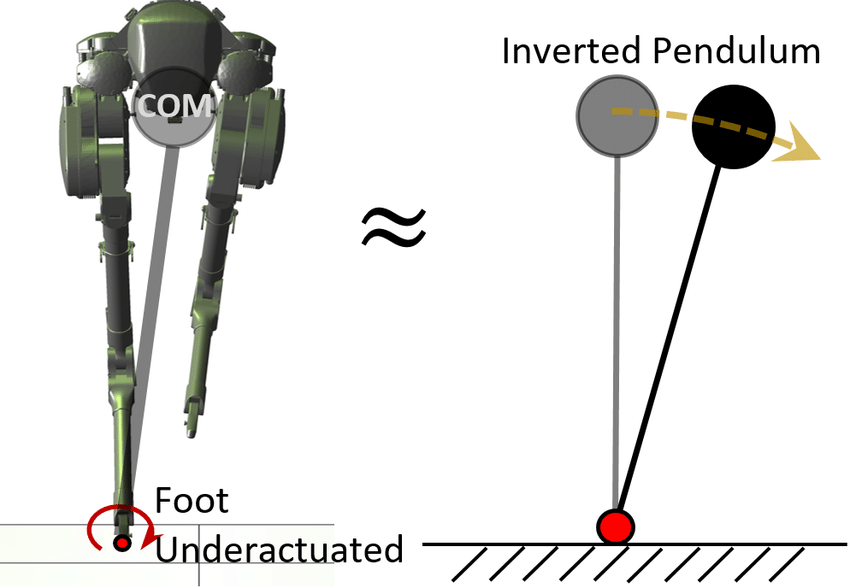
\includegraphics[height=0.65\linewidth,fbox]{underactuation-illustration-01_[xiong2021underactuated].png}
%         \end{column}
%         \begin{column}[t]{0.32\linewidth}
%             \centering
%             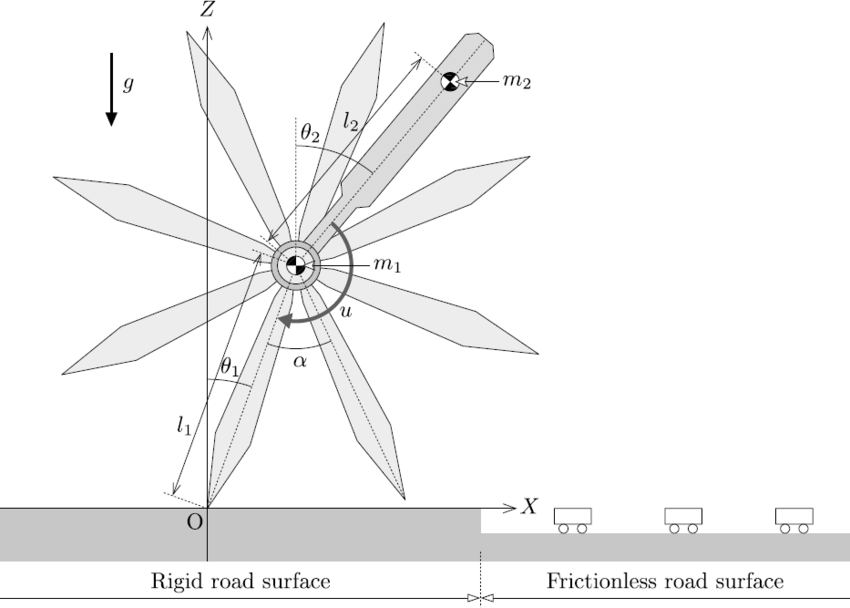
\includegraphics[height=0.65\linewidth,fbox]{underactuation-illustration-02_[asano2009stealth].png}
%         \end{column}
%         \begin{column}[t]{0.32\linewidth}
%             % \centering
%             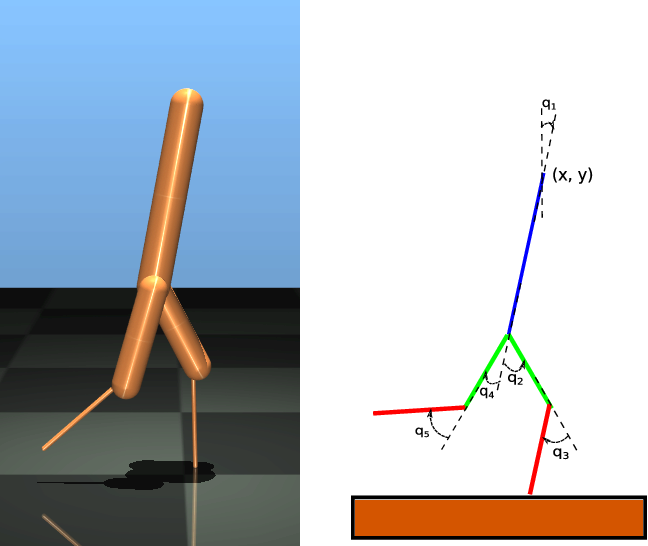
\includegraphics[height=0.65\linewidth,fbox]{underactuation-illustration-03-[talele2019mesh].png}
%         \end{column}
%     \end{columns}
% \end{frame}

\begin{frame}{Published Work}
    \begin{itemize}
        \item N. A. Ashenafi, W. Sirichotiyakul, and A. C. Satici, “Robust passivity-based control of underactuated systems via neural approximators and Bayesian inference,” in 2022 IEEE Control Systems Letters (under review), 2022. 
        \item N. A. Ashenafi and A. C. Satici, “Nonholonomic cooperative manipulation in the plane using linear complementarity formulation,” in 2021 IEEE Conference on Control Technology and Applications (CCTA). IEEE, 2021, pp. 634–639. 
        \item W. Sirichotiyakul, N. A. Ashenafi, and A. C. Satici, “Robust data-driven passivity-based control of underactuated systems via neural approximators and Bayesian inference,” in 2022 American Control Conference, 2022. 
        \item W. Sirichotiyakul, N. A. Ashenafi, and A. C. Satici, “Robust interconnection and damping assignment passivity-based control via neural Bayesian inference,” in 2022 IEEE Transactions on Automatic Control (under review), 2022.
    \end{itemize}
\end{frame}

\section{Motivation}
\centering
\frame{Motivation}

\begin{frame}{Data-Driven Control of Underactuated Systems}
    \begin{columns}
        \begin{column}[]{0.48\linewidth}
            \vspace{0.5em}
            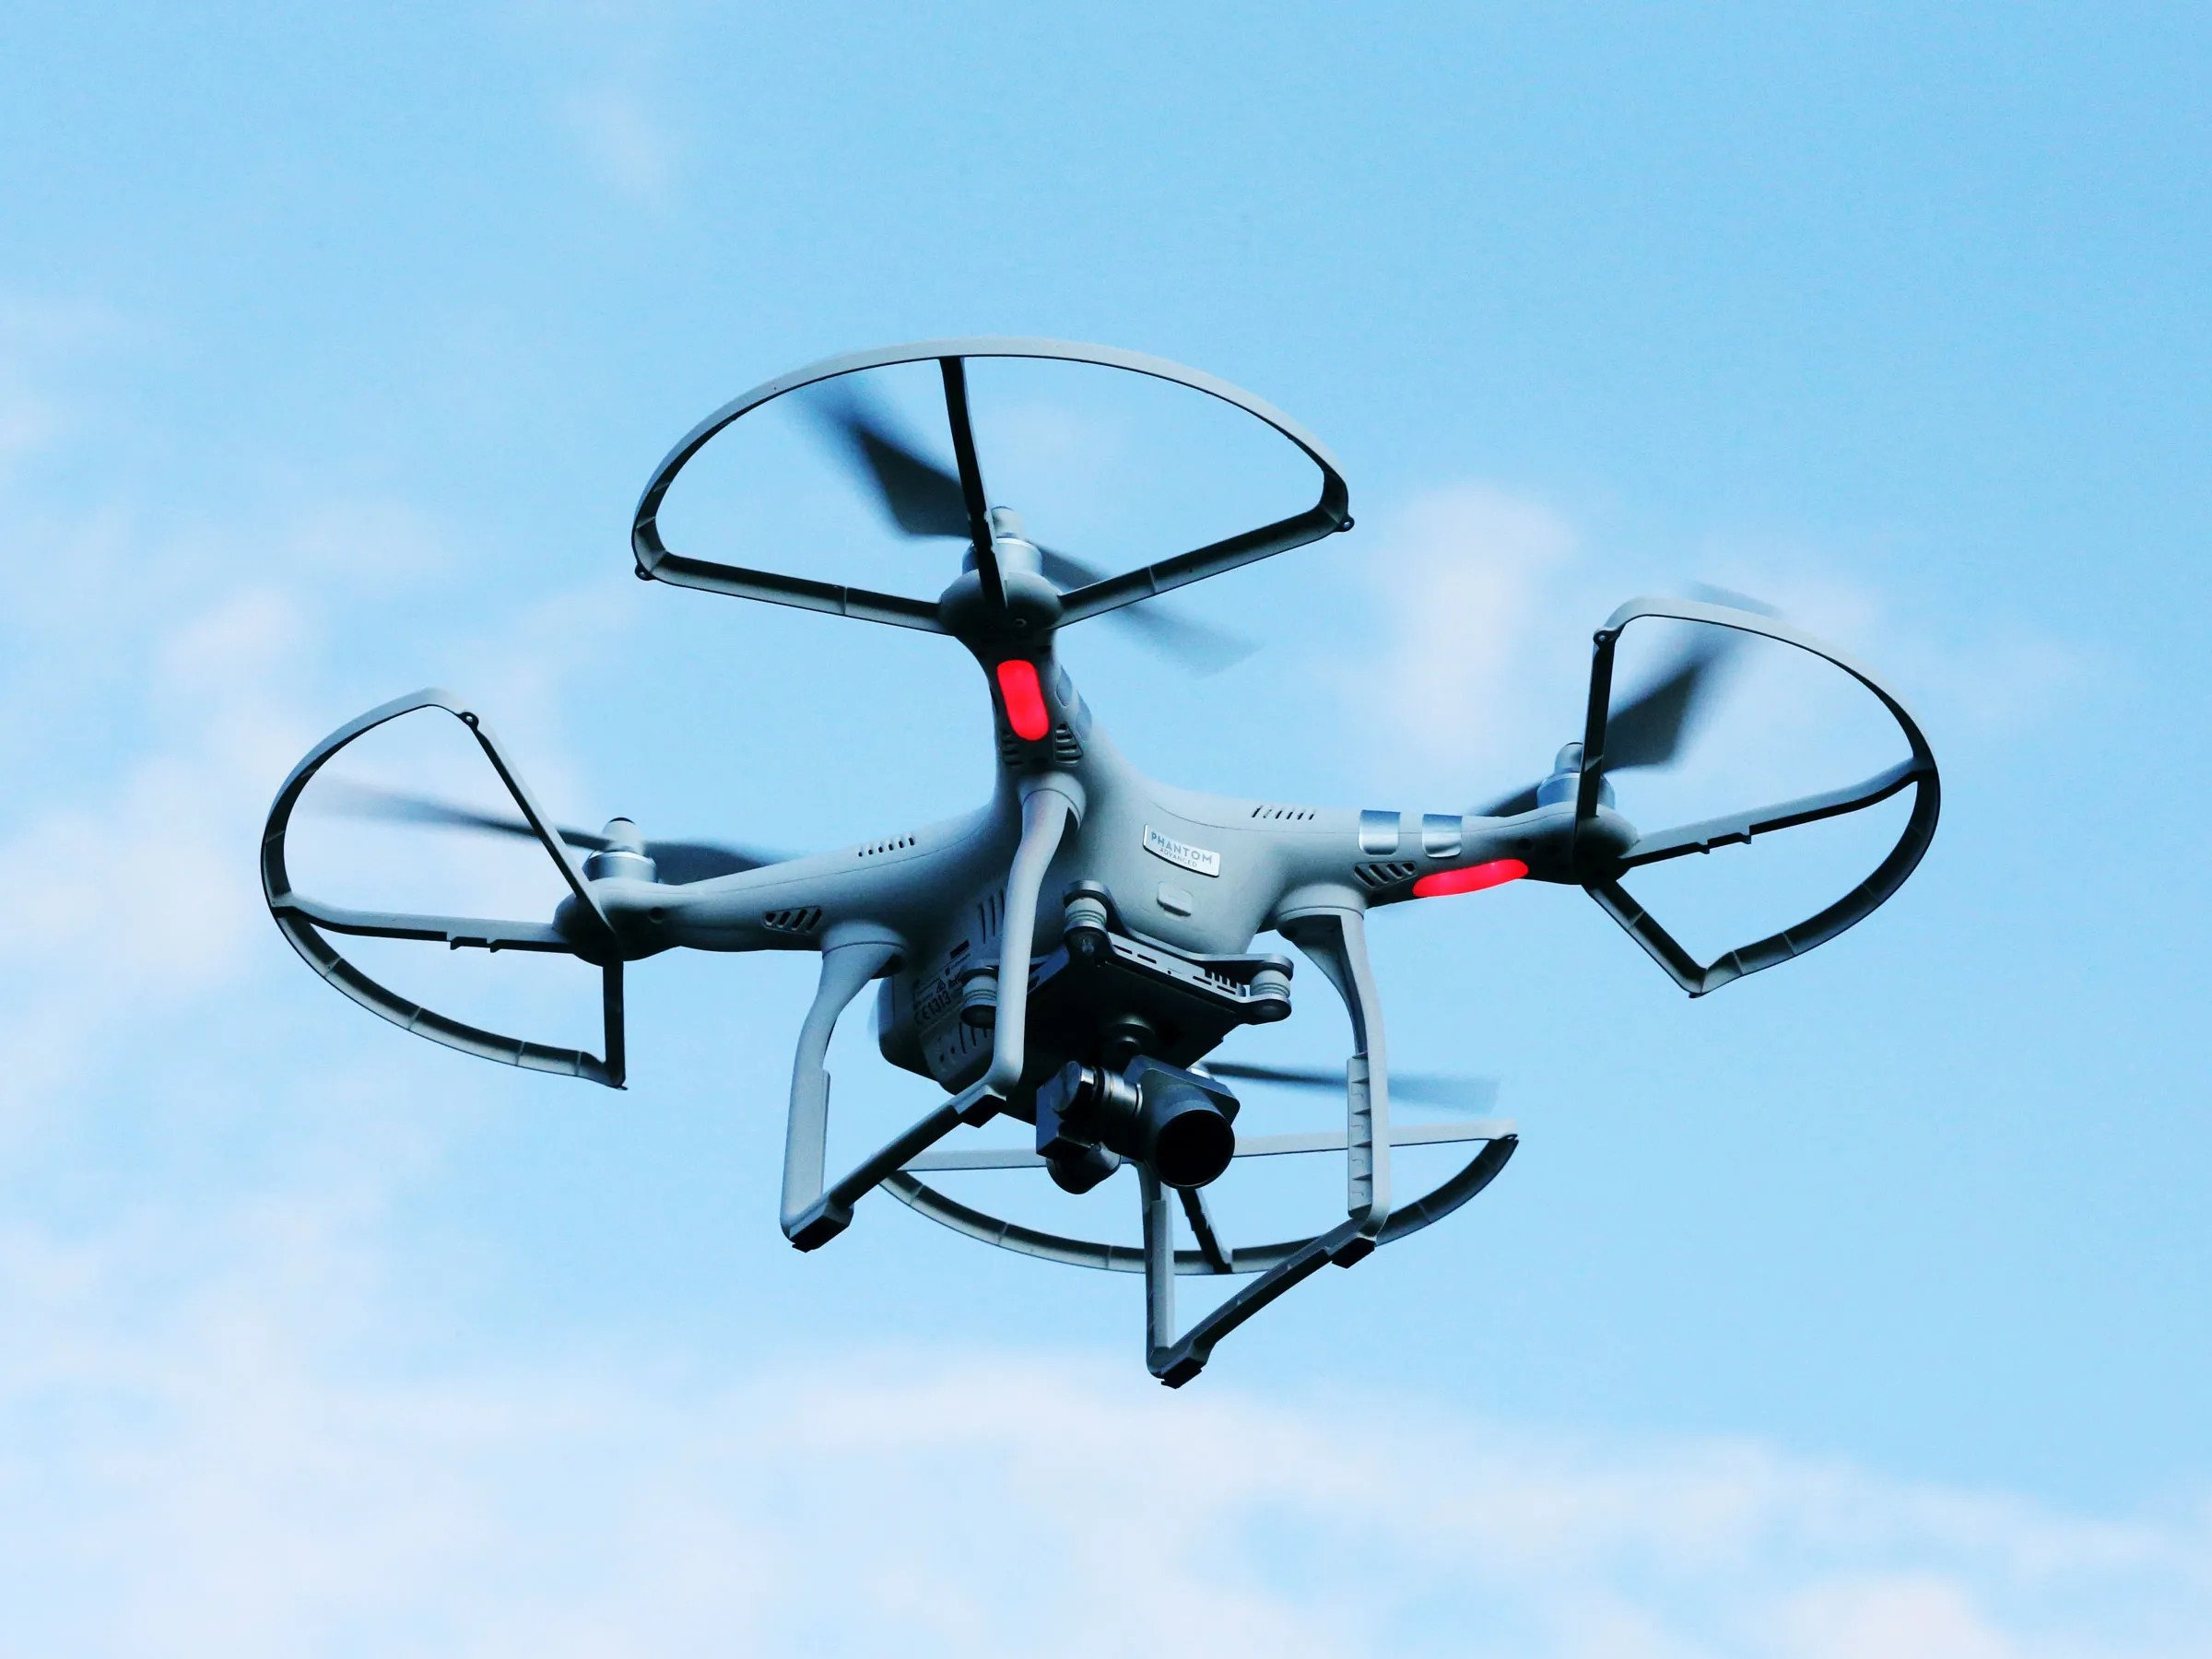
\includegraphics[width=0.4\linewidth, left]{./figures/drone.jpg}
            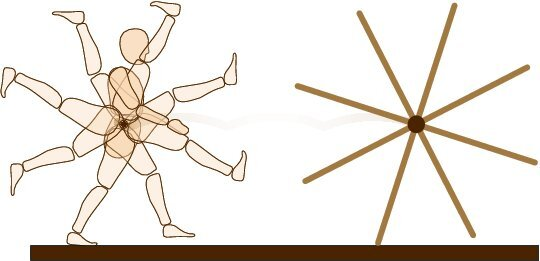
\includegraphics[width=0.5\linewidth, right]{./figures/yoyoman.jpg}
            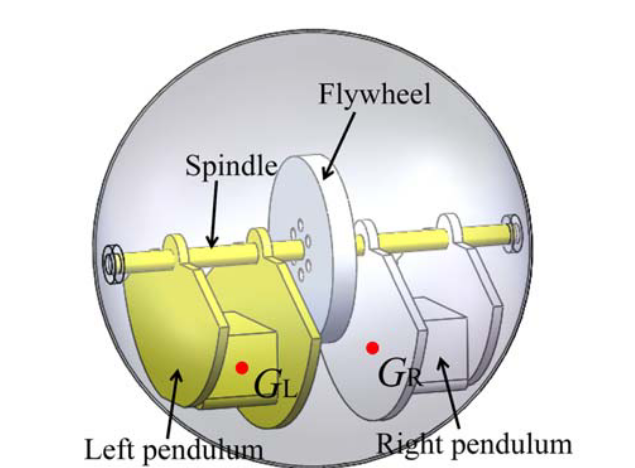
\includegraphics[width=0.5\linewidth, left]{./figures/spherical_robot.png}
        \end{column}
        \begin{column}[]{0.48\linewidth}
            \vspace{0.5em}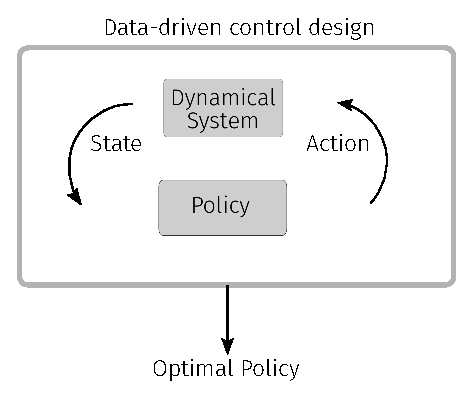
\includegraphics[]{data-driven.eps}    
        \end{column}
    \end{columns}
    \small
    \footnotetext[1]{Hu, Yibo, Yanding Wei, and Mengnan Liu. "Design and performance evaluation of a spherical robot assisted by high-speed rotating flywheels for self-stabilization and obstacle surmounting." Journal of Mechanisms and Robotics 13.6 (2021)}
\end{frame}

\begin{frame}
    \begin{columns}
        \begin{column}[t]{0.48\linewidth}
            \textbf{Learning from hardware}
            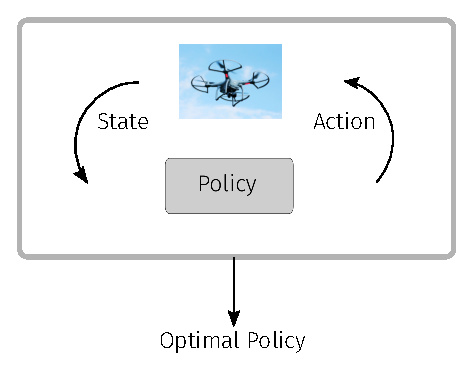
\includegraphics[]{./figures/unknown__env.eps}
            \begin{itemize}
                \item \textcolor{green}{Accurate system response}
                \item \textcolor{red}{Minimal insight to stability}
            \end{itemize}  
        \end{column}
        %\pause
        \begin{column}[t]{0.48\linewidth}
            % \vspace{1em}
            \textbf{Learning from simulation}
            \vspace{0.5em}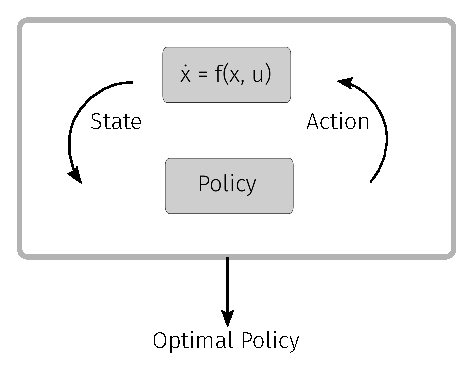
\includegraphics[]{./figures/nominal_model.eps}  
            \begin{itemize}
                \item \textcolor{green}{Provides stability analysis}
                \item \textcolor{red}{Inaccurate system response}
            \end{itemize}
        \end{column}
    \end{columns}
\end{frame}

% \begin{frame}{Our Method}
%     \begin{center} 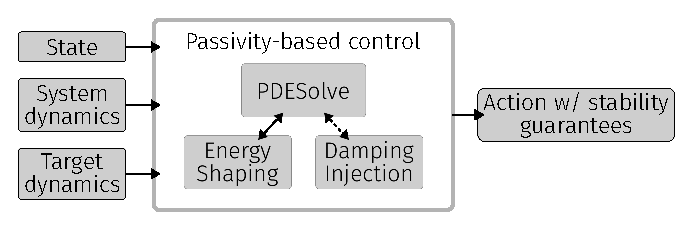
\includegraphics[]{pbc-outline.eps} \end{center}
%     \vspace{0.55em}\phantom{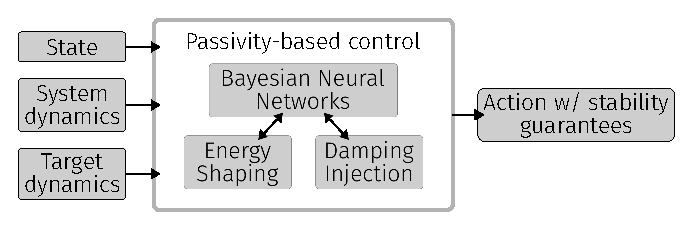
\includegraphics[]{pbc-ml-outline.eps}}
% \end{frame}
% \begin{frame}{Our Method}
%     \begin{center}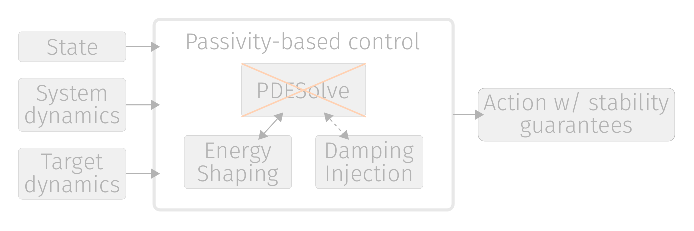
\includegraphics[]{pbc-outline-cross-fade.eps} \end{center}

%     \begin{center}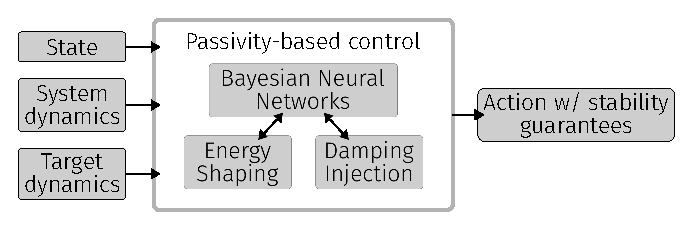
\includegraphics[]{pbc-ml-outline.eps} \end{center}
% \end{frame}

\begin{frame}{Our Method}
    \begin{columns}
        \begin{column}[]{0.48\linewidth}
            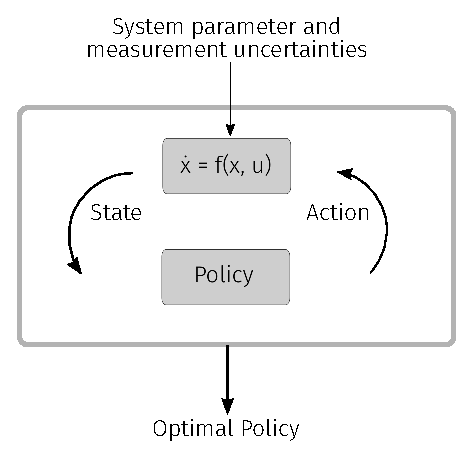
\includegraphics[width=0.9\linewidth, center]{with_uncertainty.eps}
        \end{column}
        %\pause
        \begin{column}[]{0.5\linewidth}
            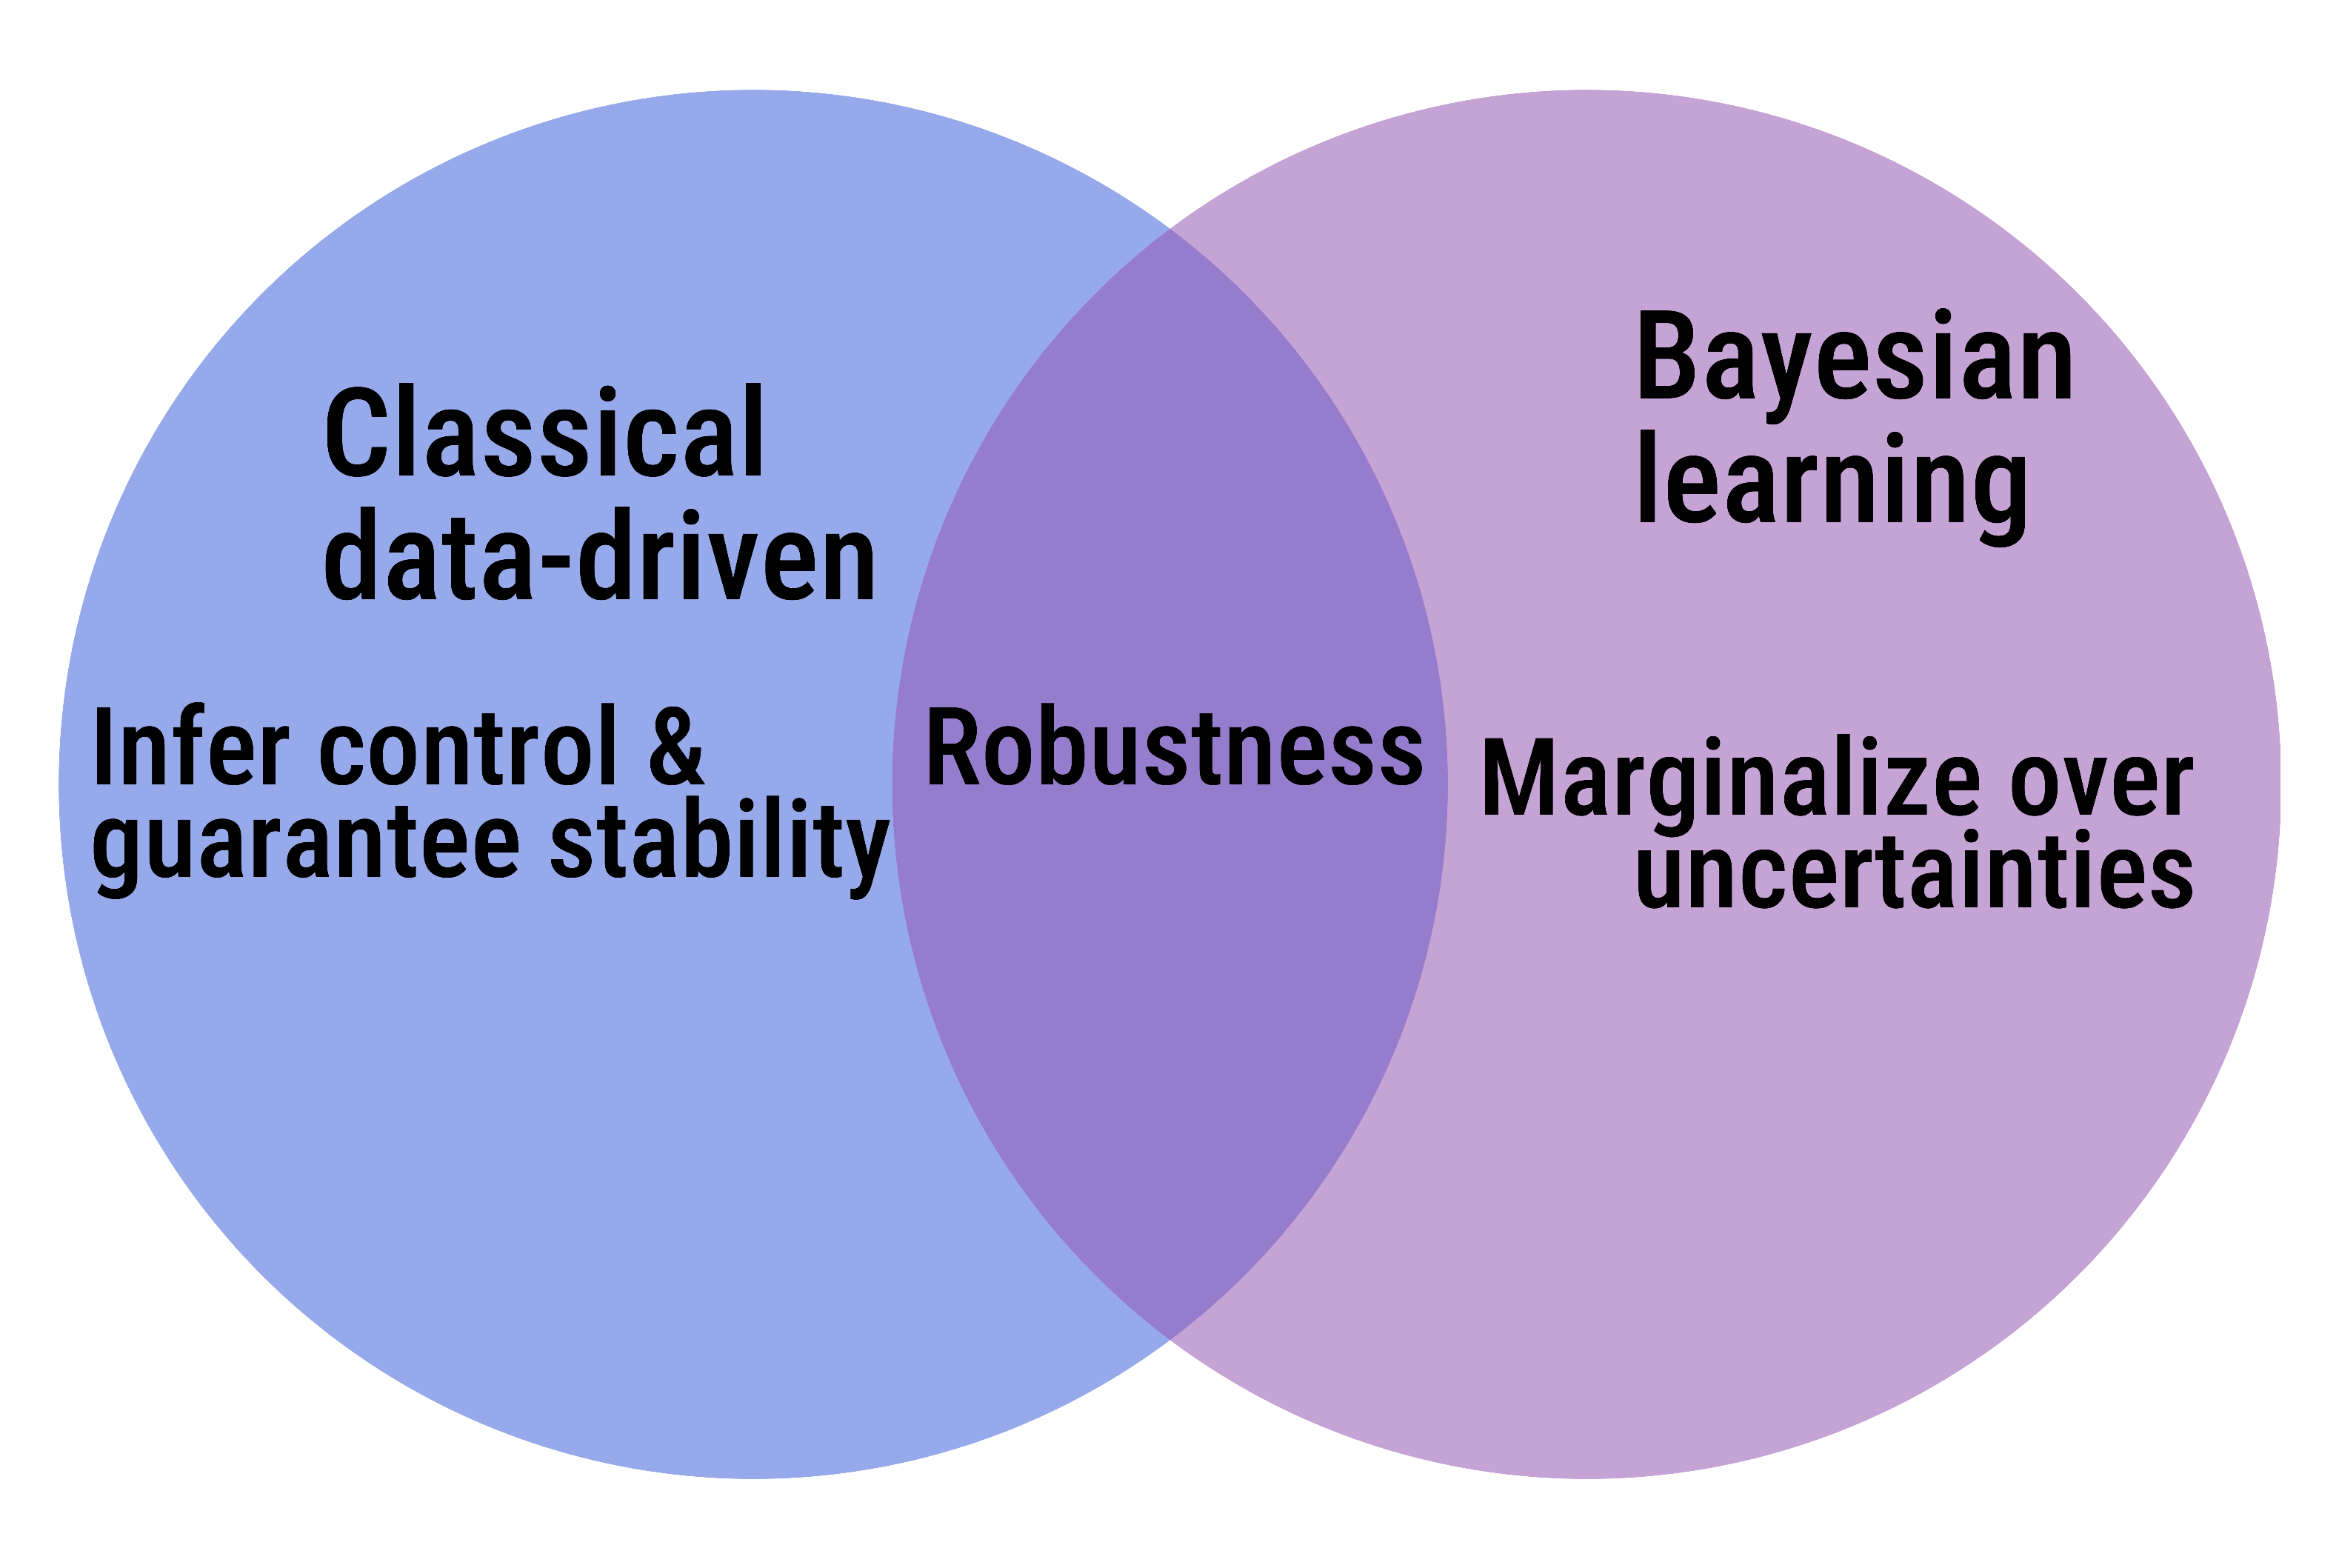
\includegraphics[width=0.8\linewidth]{venn_diagram_general.eps}
            \begin{itemize}
                \item Provides stability analysis 
                \item Desired performance for wide range of system parameters
            \end{itemize}
        \end{column}
    \end{columns}
\end{frame}


\begin{frame}{Interconnection and Damping Assignment Passivity-Based Control (\textsc{IdaPbc})}
    \begin{itemize}
        \item In the control of mechanical systems, \textsc{IdaPbc} is used to find a
        policy that overrides the overall energy of the system with a fictitious one
        with desirable characteristics.
        \begin{align*}
            H(q, p) = \frac{1}{2} p^\top M^{-1}(q)p + V(q) \hspace{0.5cm} \textcolor{red}{\xRightarrow[]{u_{es} + u_{di}}} \hspace{0.5cm} H_d(q, p) = \frac{1}{2} p^\top M_d^{-1}(q)p + V_d(q) 
        \end{align*}
    \end{itemize}
    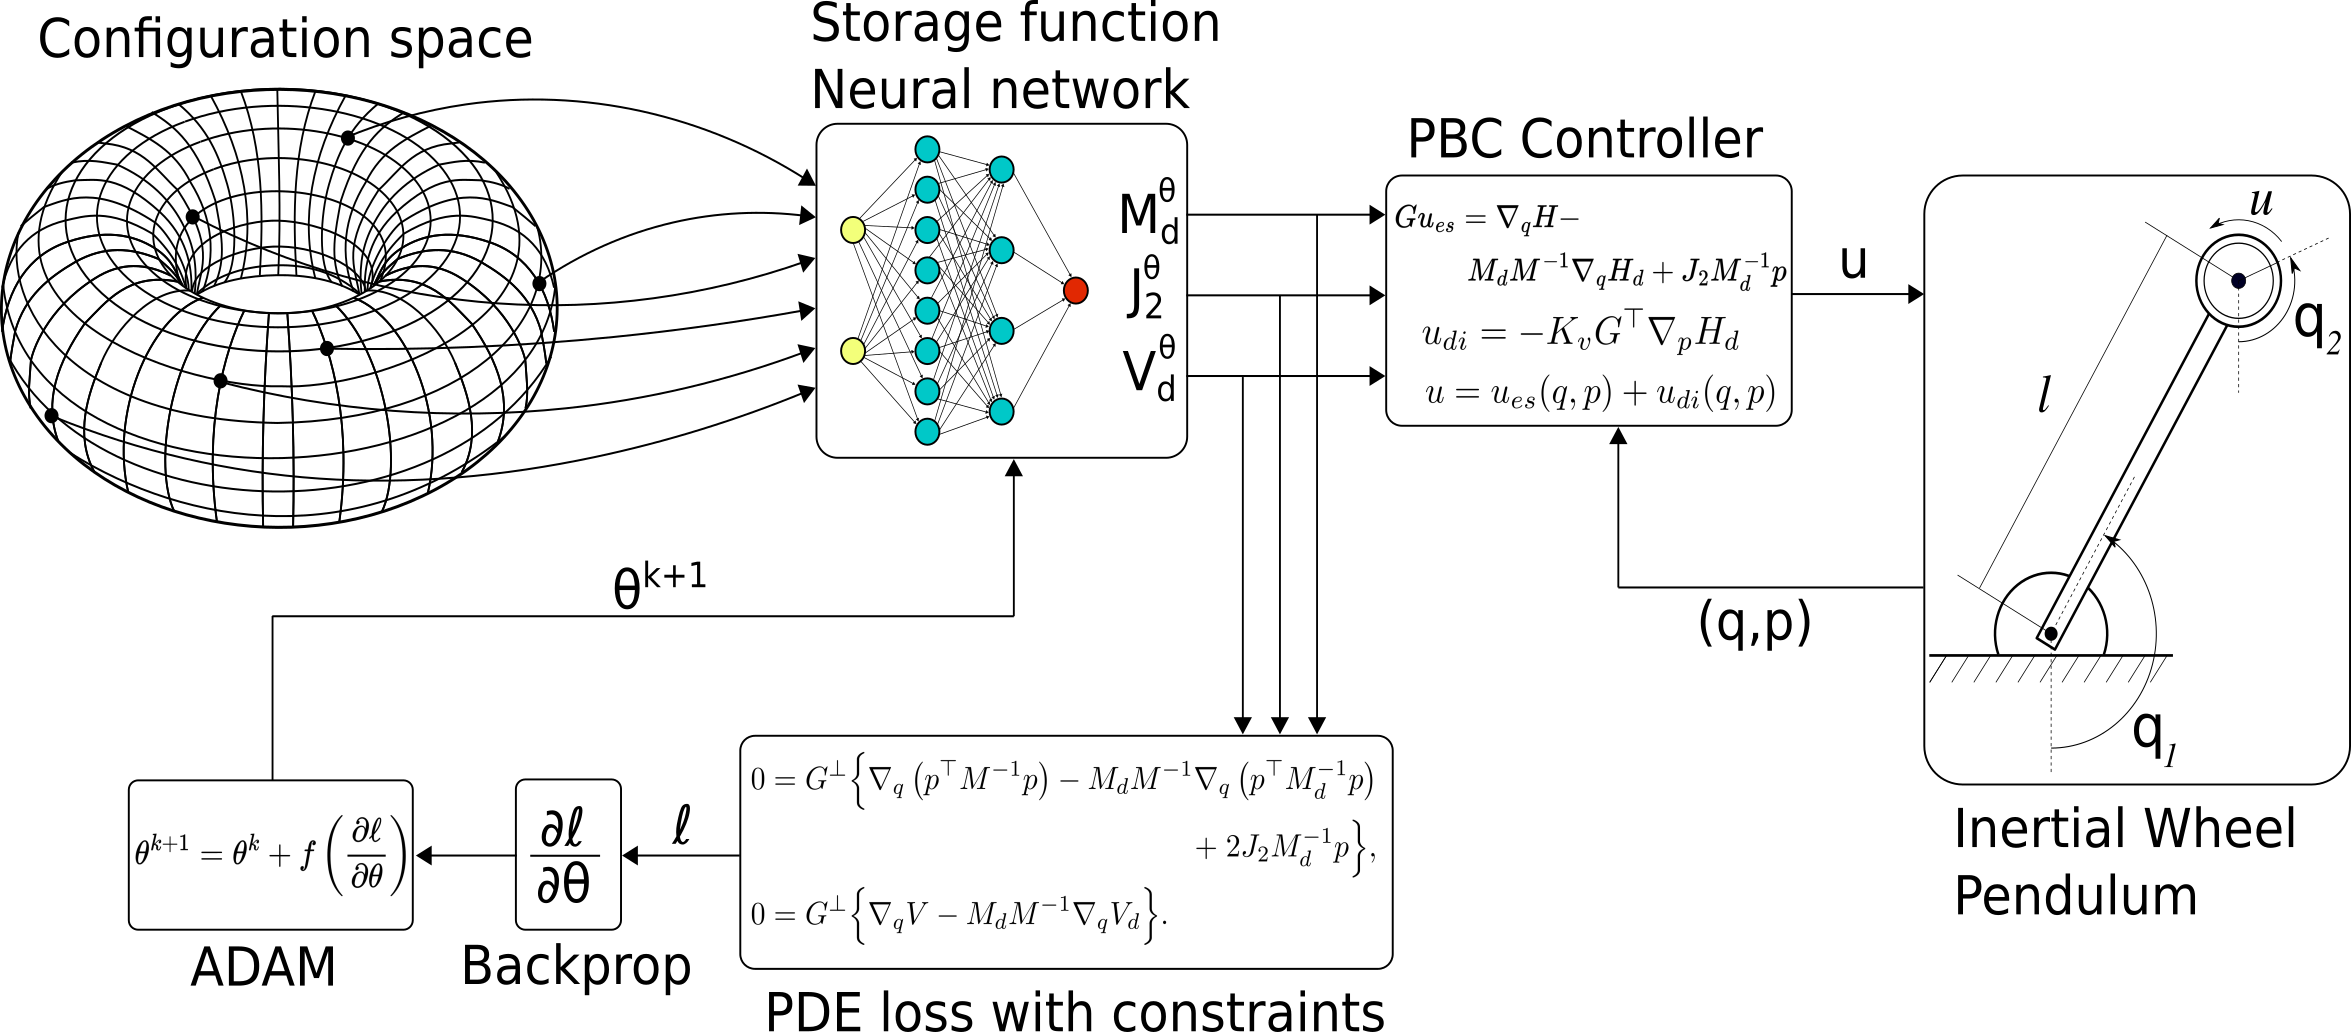
\includegraphics[width=0.7\linewidth]{nn-pbc-struct.png}
\end{frame}

\begin{frame}[fragile]
  \frametitle{ \textsc{Neural-IdaPbc}: Control Design with Stability Guarantee}
%   \begin{columns}
%   \begin{column}[c]{0.62\linewidth}
  \begin{exampleblock}{Main Learning Problem}
    %
    \begin{equation*}
      \begin{aligned}
        \underset{\theta }{\text{minimize}} 
        &&\quad J &= \left\| G^\bot \Bigl( \nabla_q H - M_d M^{-1} \nabla_q H_d + J_2 M_d^{-1} p \Bigr) \right\|^2 \\
        \text{subject to} 
        &&\quad M_d^\theta &= \big( M_d^\theta \big)^\top \succ 0, \\
        &&\quad J_2^\theta &= -\big( J_2^\theta \big)^\top, \\
        % &&\quad q^\star &= \underset{q}{\textrm{argmin}} \; V_d^\theta.  \\
        &&\quad q^\star &= \underset{q}{\text{argmin}}\; V_d^\theta.
      \end{aligned}    
      % \label{eq:finite_optim}%
    \end{equation*}
    %
    $V_d^\theta, M_d^\theta, J_2^\theta$ are 
    %\textcolor{green}{surrogates}, 
    parametrized by neural networks.
  \end{exampleblock}
  
%   \begin{itemize}
    % \setlength{\itemindent}{-1em}
    % \addtolength{\itemindent}{-2em}
    % \item %
    % $(V_d^\theta, M_d^\theta, J_2^\theta) \to$ make the target function $F(x;\theta)$
  
    % \item For $J < \epsilon$, $\exists t \in (0, \infty)$ s.t. $\left\| x(t) - x^\star \right\| < \delta$
    % \begin{itemize}
    %   \setlength{\itemindent}{-1.5em}
    %   \item Continuous dependence on parameters of ODE solutions
    % \end{itemize}
%   \end{itemize}
%   \end{column}    
  
%   \begin{column}[c]{0.36\linewidth}
 
%   \end{column}
%   \end{columns}
\end{frame}